\documentclass[11pt,oneside,letterpaper]{article}

% graphicx package, useful for including eps and pdf graphics
\usepackage{graphicx}
\DeclareGraphicsExtensions{.pdf,.png,.jpg}

% basic packages
\usepackage{color} 
\usepackage{parskip}
\usepackage{float}

% text layout
\usepackage{geometry}
\geometry{textwidth=15cm} % 15.25cm for single-space, 16.25cm for double-space
\geometry{textheight=22cm} % 22cm for single-space, 22.5cm for double-space

% helps to keep figures from being orphaned on a page by themselves
\renewcommand{\topfraction}{0.85}
\renewcommand{\textfraction}{0.1}

% bold the 'Figure #' in the caption and separate it with a period
% Captions will be left justified
\usepackage[labelfont=bf,labelsep=period,font=small]{caption}

% review layout with double-spacing
%\usepackage{setspace} 
%\doublespacing
%\captionsetup{labelfont=bf,labelsep=period,font=doublespacing}

% cite package, to clean up citations in the main text. Do not remove.
\usepackage{cite}
%\renewcommand\citeleft{(}
%\renewcommand\citeright{)}
%\renewcommand\citeform[1]{\textsl{#1}}

% Remove brackets from numbering in list of References
\renewcommand\refname{\large References}
\makeatletter
\renewcommand{\@biblabel}[1]{\quad#1.}
\makeatother

\usepackage{authblk}
\renewcommand\Authands{ \& }
\renewcommand\Authfont{\normalsize \bf}
\renewcommand\Affilfont{\small \normalfont}

% notation
\usepackage{amsmath}
\usepackage{amssymb}
\newcommand{\virus}{\mathbf{x}}						% virus coordinate
\newcommand{\serum}{\mathbf{y}}						% serum coordinate
\newcommand{\viruses}{\mathbf{X}}					% set of virus coordinates
\newcommand{\sera}{\mathbf{Y}}						% set of serum coordinates
\newcommand{\ve}{v}									% virus effect
\newcommand{\se}{s}									% serum effect
\newcommand{\ves}{\mathbf{v}}						% set of virus effects
\newcommand{\ses}{\mathbf{s}}						% set of serum effects
\newcommand{\point}{f_{\scriptscriptstyle \vert}}	% point likelihood
\newcommand{\threshold}{f_{\textstyle \lrcorner}}	% threshold likelihood
\newcommand{\interval}{f_{\sqcup}}					% interval likelihood
\newcommand{\mdssd}{\varphi}						% MDS standard deviation
\newcommand{\virussd}{\sigma_x}						% Virus / Diffusion standard deviation
\newcommand{\serumsd}{\sigma_y}						% Serum standard deviation
\newcommand{\tree}{\tau}							% Phylogeny
\newcommand{\vn}{n}									% Number of viruses
\newcommand{\sn}{k}									% Number of sera
\newcommand{\node}{\mathbf{z}}						% Internal node in phylogeny
\newcommand{\normal}{\mathcal{N}}					% Normal distribution
\setlength{\arraycolsep}{2pt}
\newcommand{\smalltwomatrix}[2]{\scriptsize \Big( \begin{matrix} #1 \\ #2 \end{matrix} \Big)}				% pretty inline matrix 
\newcommand{\smallfourmatrix}[4]{\scriptsize \Big( \begin{matrix} #1 & #2 \\ #3 & #4 \end{matrix} \Big)}	% pretty inline matrix 
\newcommand{\twomatrix}[2]{\left( \begin{matrix} #1 \\ #2 \end{matrix} \right)}								% pretty inline matrix 
\newcommand{\fourmatrix}[4]{\left( \begin{matrix} #1 & #2 \\ #3 & #4 \end{matrix} \right)}					% pretty inline matrix 

% comments
\usepackage{ulem}
\definecolor{blue}{rgb}{0.324,0.609,0.708}
\definecolor{purple}{rgb}{0.459,0.109,0.538}
\def\tb#1#2{\sout{#1} \textcolor{purple}{#2}} 
\def\tbc#1{\textcolor{purple}{[#1]}}
\def\ms#1#2{\sout{#1} \textcolor{blue}{#2}} 
\def\msc#1{\textcolor{blue}{[#1]}}

%%% TITLE %%%
\title{\vspace{1.0cm} \Large \bf 
Revealing the competitive dynamics of influenza viruses through evolutionary cartography \\
or \\
Charting antigenic drift and evolutionary success of seasonal influenza lineages \\
or \\
Integrating influenza antigenic dynamics with molecular evolution \\
or \\
Cartographic analysis of antigenic dynamics and evolutionary success of seasonal influenza lineages \\
or \\
Integrating antigenic cartography and molecular evolution to characterize predictors of evolutionary success of seasonal influenza lineages 
}

\author[1]{Trevor Bedford}
\author[2,3,4]{Marc A. Suchard}
\author[5]{Philippe Lemey}
\author[1]{Gytis Dudas}
\author[6]{Victoria Gregory}
\author[6]{Alan J. Hay}
\author[6]{John W. McCauley}
\author[7]{Colin Russell}
\author[7,8]{Derek Smith}
\author[1,9]{Andrew Rambaut}

\affil[1]{Institute of Evolutionary Biology, University of Edinburgh, Edinburgh, UK}
\affil[2]{Department of Biomathematics, David Geffen School of Medicine at UCLA, University of California, Los Angeles CA, USA}
\affil[3]{Department of Human Genetics, David Geffen School of Medicine at UCLA, University of California, Los Angeles CA, USA}
\affil[4]{Department of Biostatistics, UCLA Fielding School of Public Health, University of California, Los Angeles CA, USA}
\affil[5]{Department of Microbiology and Immunology, Katholieke Universiteit Leuven, Leuven, Belgium}
\affil[6]{Division of Virology, MRC National Institute for Medical Research, Mill Hill, London, UK}
\affil[7]{Department of Zoology, University of Cambridge, Cambridge, UK}
\affil[8]{Department of Virology, Erasmus Medical Centre, Rotterdam, Netherlands}
\affil[9]{Fogarty International Center, National Institutes of Health, Bethesda, MD, USA}

\date{}

\begin{document}

\maketitle

%%% ABSTRACT %%%
\section*{Abstract}

Influenza viruses undergo continual antigenic evolution allowing mutant viruses to evade immunity acquired by the host population to previous virus strains.
Antigenic phenotype is often assessed through pairwise measurement of cross-reactivity between influenza strains using the hemagglutination inhibition (HI) assay.
Here, we extend previous approaches to antigenic cartography, which seeks to place strains on an antigenic map, such that distances on this map best recapitulate titers observed across multiple HI assays.
In our model, we simultaneously characterize antigenic and genetic evolution by including an evolutionary model in which antigenic location diffuses over a shared virus phylogeny.
Using HI data for influenza lineages A/H3N2, A/H1N1, B/Victoria and B/Yamagata, we determine average rates of antigenic drift for each clade, as well as year-to-year variability in the rate of drift.
Through comparison with epidemiological data, we show that antigenic drift influences overall incidence across clades, and demonstrate a year-to-year correlation between drift and incidence.
We investigate the selective underpinnings for differing antigenic dynamics across clades and show that A/H3N2 benefits from both a higher influx of new antigenic mutations and also from more efficient conversion of antigenic variation into fixed differences relative to other influenza clades.
This work does much to elucidate the competitive dynamics of influenza lineages, but also makes possible substantial future advances in influenza and other antigenically-variable pathogens by providing a model that intimately combines molecular and antigenic evolution.

\pagebreak

%%% INTRODUCTION %%%
\section*{Introduction}

Seasonal influenza infects between 10\% and 20\% of the human population every year, causing 250,000 to 500,000 deaths annually \cite{flufactsheet}. 
While individuals develop long-lasting immunity to particular influenza strains after infection, antigenic mutations to the influenza virus genome result in proteins that are recognized to a lesser degree by the human immune system, leaving individuals susceptible to future infection. 
The influenza virus population continually evolves in antigenic phenotype in a process known as antigenic drift. 
A large proportion of the disease burden of influenza stems from antigenic drift; it is why vaccines remain only transiently effective. 
A thorough understanding of the process of antigenic drift is essential to public health efforts to control mortality and morbidity through the use of a seasonal influenza vaccine.

Before 2009, there were four major clades of influenza circulating within the human population: A/H3N2, A/H1N1, B/Victoria and B/Yamagata. 
In the case of influenza A, subtypes A/H3N2 and A/H1N1 refer to the genes, hemagglutinin (H or HA) and neuraminidase (N or NA), that are primarily responsible for the antigenic character of a strain. 
In the case of influenza B, B/Vic and B/Yam refer to antigenically distinct lineages which diverged from one prior to 1980 \cite{Rota92}.
Mutations to the HA1 region of the hemagglutinin protein are thought to drive the majority of antigenic drift in the influenza virus \cite{Nelson07NatRevGenet}. 
Experimental characterization of antigenic phenotype is possible through the hemagglutination inhibition (HI) assay \cite{Hirst43}, which measures the cross-reactivity of one virus strain to serum raised against another strain through challenge or vaccination. 
Sera from older strains react poorly with more evolved viruses resulting in new strains having a transmission advantage over previously established strains.
HI assays have shown there to be little to no cross-reactivity between influenza clades A/H3N2, A/H1N1, B/Vic and B/Yam \cite{Hay01}.

The results of many HI assays across a multitude of virus strains can be combined to yield a two-dimensional map, quantifying antigenic similarity and distance \cite{Smith04}. 
The antigenic map of influenza A/H3N2 has shown largely linear movement of the influenza virus population since its introduction in 1968. 
Evolution of antigenic phenotype appears punctuated with periods of stasis interspersed by periods of more rapid innovation, while genetic evolution appears more continuous \cite{Smith04}, suggesting that a relatively small number of genetic changes or combinations of genetic changes may drive changes in antigenic phenotype. 
The process of antigenic drift results in the rapid turnover of the virus population. 
Although mutation occurs rapidly, standing genetic diversity is low and phylogenetic analysis shows a characteristically `spindly' tree with a single predominant trunk lineage and transitory side branches that persist for only 1--5 years \cite{Fitch97}.

Previously, the antigenic and genetic patterns of influenza evolution have been analyzed essentially in isolation. 
An antigenic map is constructed from a panel of HI measurements, and a phylogenetic tree is constructed from sequence data. 
However, the opportunity for a combined approach exists as both the antigenic map and the phylogenetic tree often contain many of the same isolates. 
Here, we implement a flexible Bayesian approach to jointly characterize the antigenic and genetic evolution of the influenza virus population. 
We apply this approach to investigate the dynamics of clades A/H3N2, A/H1N1, B/Vic and B/Yam. 

%%% RESULTS %%%
\section*{Results and Discussion}

\subsection*{Antigenic and evolutionary cartography}

In order to assess patterns of antigenic evolution among influenza strains, we implemented a Bayesian probabilistic analog of multidimensional scaling (MDS), referred to here as BMDS (see Methods).
In this model, viruses and sera are given $N$-dimensional locations, thus specifying an `antigenic map', such that distances between viruses and sera in this space are inversely proportional to cross-reactivity.
In the BMDS model, a map distance of one antigenic unit translates to an expectation of a 2-fold drop in HI titer between virus and sera.
Maps that produce pairwise distances most congruent with the observed titers will have a high likelihood and will be favored by the BMDS model.
We integrate over sources of uncertainty, such as antigenic locations, in a flexible Bayesian fashion.
We apply this model to HI measurements of virus isolates against post-infection ferret sera for influenza A/H3N2, A/H1N1, B/Vic and B/Yam (see Methods).

We test model performance by constructing training datasets representing 90\% of the HI measurements for each of the four influenza lineages and test datasets representing the remaining 10\% of the measurements for each lineage. 
By fitting the BMDS model to the training dataset, we are able to predict HI titers in the test dataset and compare these predicted titers to observed titers. 
We begin with a BMDS analog of the model used by Smith et al.\ \cite{Smith04}, in which viruses and sera are represented as 2D locations, expected titer is relative to the maximum titer of a particular ferret serum and virus and serum locations follow a diffuse prior.
We find that this model performs well, yielding an average absolute predictive error of between 0.79 and 0.95 log$_2$ HI titers across influenza lineages (model 1; Table \ref{errortable}).
We extend this model to include a time-informed prior that models the process of antigenic drift, in which virus and serum locations  along dimension 1 increase with date of virus or serum sampling, resulting in a small improvement in predictive error (model 2; Table \ref{errortable}).

%%% errortable %%%
\begin{table}[h]
	\centering
	\caption{\textbf{Average absolute prediction error of log$_2$ HI titer for test data across models and datasets.}}
	\label{errortable}	
	\makebox[\textwidth][c]{
	\begin{tabular}{ c c c c c c c c c } 
	\hline
	\multicolumn{5}{c}{} 	&	\multicolumn{4}{c}{Test error}  \\
	Model	&	Dimen 	& 	Serum effects 	&	Virus effects	& Location Prior	& 	A/H3N2	& 	A/H1N1	& 	B/Vic	& 	B/Yam	\\
	\hline		
	1		&	2D 		&	Fixed 			&	None			& Uninformed		&	0.93 	&	0.78 	&	0.80	&	0.93	\\
	2		&	2D 		&	Fixed			&	None			& Drift				&	0.91 	&	0.74 	&	0.77	&	0.83	\\	
	3		&	1D 		&	Fixed			&	None			& Drift				&	1.07	&	0.92	&	0.94	&	1.08	\\		
	4		&	3D 		&	Fixed			&	None			& Drift				&	0.91	&	0.74 	&	0.79	&	0.84	\\
	5		&	4D 		&	Fixed			&	None			& Drift				&	0.95	&	0.75 	&	0.81	&	0.86	\\
	6		&	5D 		&	Fixed			&	None			& Drift				&	0.99	&	0.76 	&	0.84	&	0.88	\\				
	7		&	2D 		&	Estimated		&	Estimated		& Drift				&	0.77	&	0.71 	&	0.65	&	0.73	\\	
	8		&	2D 		&	Estimated		&	Estimated		& Diffusion/Drift	&	0.76	&	0.71 	&	0.64	&	0.72	\\		
	\hline
	\end{tabular}	
	}
\end{table}

We find that decreasing dimensionality to a single antigenic dimension results in a substantially less predictive model (model 3; Table \ref{errortable}), and that increasing dimensionality to three dimensions is equal or slightly worse in predictive power (model 4; Table \ref{errortable}).
Increasing dimensionality further to four or five dimensions results in continued declines in predictive power (models 5 and 6; Table \ref{errortable}).
Consequently, we specify a two dimensional model in all subsequent analyses.
The finding of a low-dimensional map across influenza lineages extends previous studies in A/H3N2 \cite{Smith04} and remains an interesting empirical observation.
We extend the 2D model by estimating the strength of overall reactivity of each serum rather than fixing this at its maximum titer, and additionally, by estimating the strength of reactivity of each virus isolate.
We refer to these estimates as serum effects and virus effects, respectively.
We find that including these effects decreases test error further, ranging from an improvement of 0.03 in A/H1N1 to an improvement of 0.14 in A/H3N2 (model 7; Table \ref{errortable}).

Previous work on influenza antigenic and genetic evolution has examined antigenic and genetic patterns in isolation, and then compared the results to assess congruence of these two aspects of evolution \cite{Hay01,Smith04,Russell08}. 
Here, we simultaneously model antigenic and genetic evolution by adopting an evolutionary diffusion process \cite{Lemey10}, wherein a virus's antigenic character state evolves along branches of phylogenetic tree according to a Brownian motion process (see Methods).
The diffusion process acts as a prior on virus locations, so that genetically similar viruses are expected to share similar antigenic locations.
We include sequence data for A/H3N2, A/H1N1, B/Vic and B/Yam to estimate this diffusion process, and find a small increase in predictive accuracy when including covariance induced by the phylogenetic diffusion (model 8; Table \ref{errortable}).
Additionally, modeling antigenic diffusion has the advantage of allowing direct correlation of evolutionary outcomes with changes in antigenic phenotype.

We find that the average absolute error in predicted log$_2$ HI titer is nearly constant with antigenic distance (Figure~\ref{error_by_distance_and_year}A), thus supporting our model assumption that drop in log$_2$ titer is proportional to the Euclidean distance separating viruses and sera on the antigenic map.
Additionally, we find that absolute error in predicted titer is nearly constant with time (Figure~\ref{error_by_distance_and_year}B).
Antigenic locations inferred by the model are well resolved; estimates of antigenic distance between pairs of viruses show relatively little variation across the posterior.
We estimate that virus distances have, on average, a 50\% credible interval of $\pm0.45$ antigenic units for A/H3N2, $\pm0.57$ units for A/H1N1, $\pm0.76$ units for B/Vic, and $\pm0.65$ units for B/Yam.

\subsection*{Antigenic evolution across influenza lineages}

Through our analysis, we reveal the antigenic, as well as evolutionary, relationships among viruses in influenza A/H3N2, A/H1N1, B/Vic and B/Yam, quantifying both antigenic and evolutionary distances between strains (Figure~\ref{map}).
Over the time period of 1968 to 2011, influenza A/H3N2 shows substantially more antigenic evolution than is exhibited by A/H1N1 over the course of 1977 to 2009 or B/Vic and B/Yam over the course of 1986 to 2011.
We observe prominent antigenic clusters in A/H3N2 and A/H1N1, but less prominent, though still apparent, clustering in B/Vic and B/Yam.
Antigenic clusters show high genetic similarity, so that we observe very few mutation events leading to each cluster, rather than the repeated emergence of clusters.
This analysis makes the fate of antigenic clusters obvious, with two clusters in A/H3N2 (Texas/77 and Beijing/89) appearing to be evolutionary dead-ends.

%%% map %%%
\begin{figure}[h]
	\centering		
	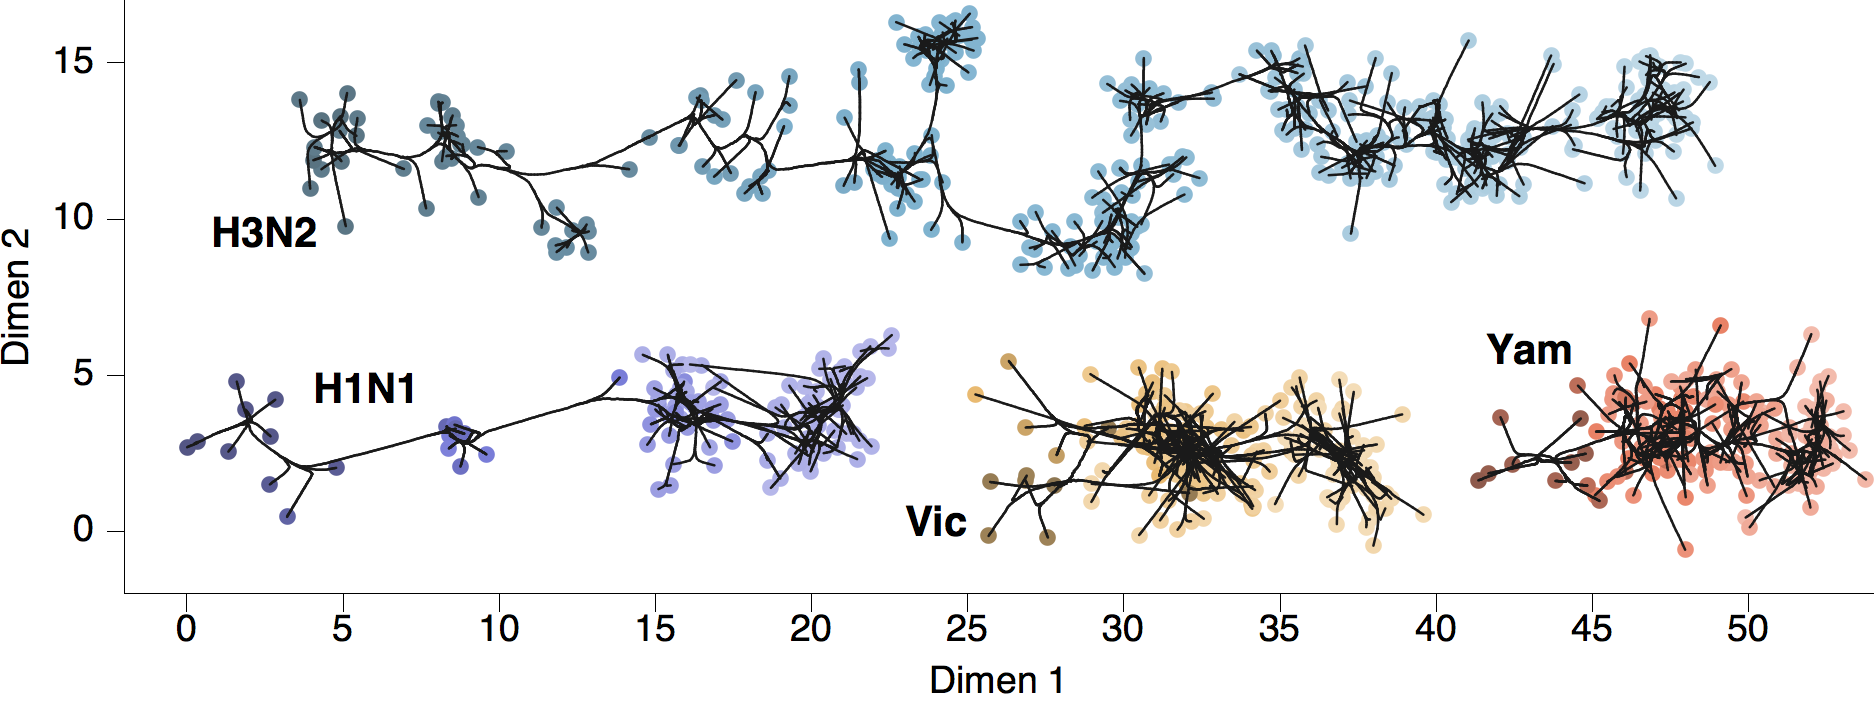
\includegraphics[width=1.0\textwidth]{figures/map}
	\caption{\textbf{Antigenic locations of A/H3N2, A/H1N1, B/Vic and B/Yam viruses showing evolutionary relationships between virus samples.} 
	Circles represent a posterior sample of virus locations and have been shaded based on year of isolation.
	Antigenic units represent two-fold dilutions of the HI assay.
	Distances between clades, e.g.\ A/H3N2 and A/H1N1, are arbitrary.
	Lines represent mean posterior diffusion paths when virus locations are fixed.} 
	\label{map} 
\end{figure}

HI assays lack sensitivity beyond a certain point, so that for A/H3N2, cross-reactive measurements only exist between strains sampled at most 11 years apart, leaving only threshold titers, e.g.\ `$<$40', in more temporally distant comparisons.  
Because of the threshold of sensitivity of the HI assay, it's impossible to distinguish a linear trajectory in 2D antigenic space, from a slightly curved trajectory, so long as the curve does not bring antigenic phenotype full circle to have cross-reactive measurements between temporally distant strains.
To solve this problem of identifiability, we assumed a weak prior that favors linear movement in the 2D antigenic space (present in models 2 through 8; Table \ref{errortable}), with the slope of the linear relationship and the precision of the relationship incorporated into the Bayesian model (see Methods).
Because of this, we interpret antigenic locations locally rather than globally.
We can determine the rate of antigenic movement of virus lineages without knowing the larger configuration that the movement occurs under.
 
We find that influenza A/H3N2 evolved along antigenic dimension 1 at a rate of $\beta=1.01$ antigenic units per year, with a 95\% highest posterior density (HPD) interval of 0.98--1.04 (Figure~\ref{drift}).
However, we observe occasional large jumps in antigenic phenotype (Figure~\ref{drift}), corresponding to cluster transitions identified by Smith et al. \cite{Smith04}.  
Most variation is contained within the first antigenic dimension, but dimension 2 occasionally shows variation when two antigenically distinct lineages emerge and transiently coexist (Figure~\ref{map}), as is the case with the previously identified Beijing/89 and Beijing/92 clusters.

%%% drift %%%
\begin{figure}[h]
	\centering		
	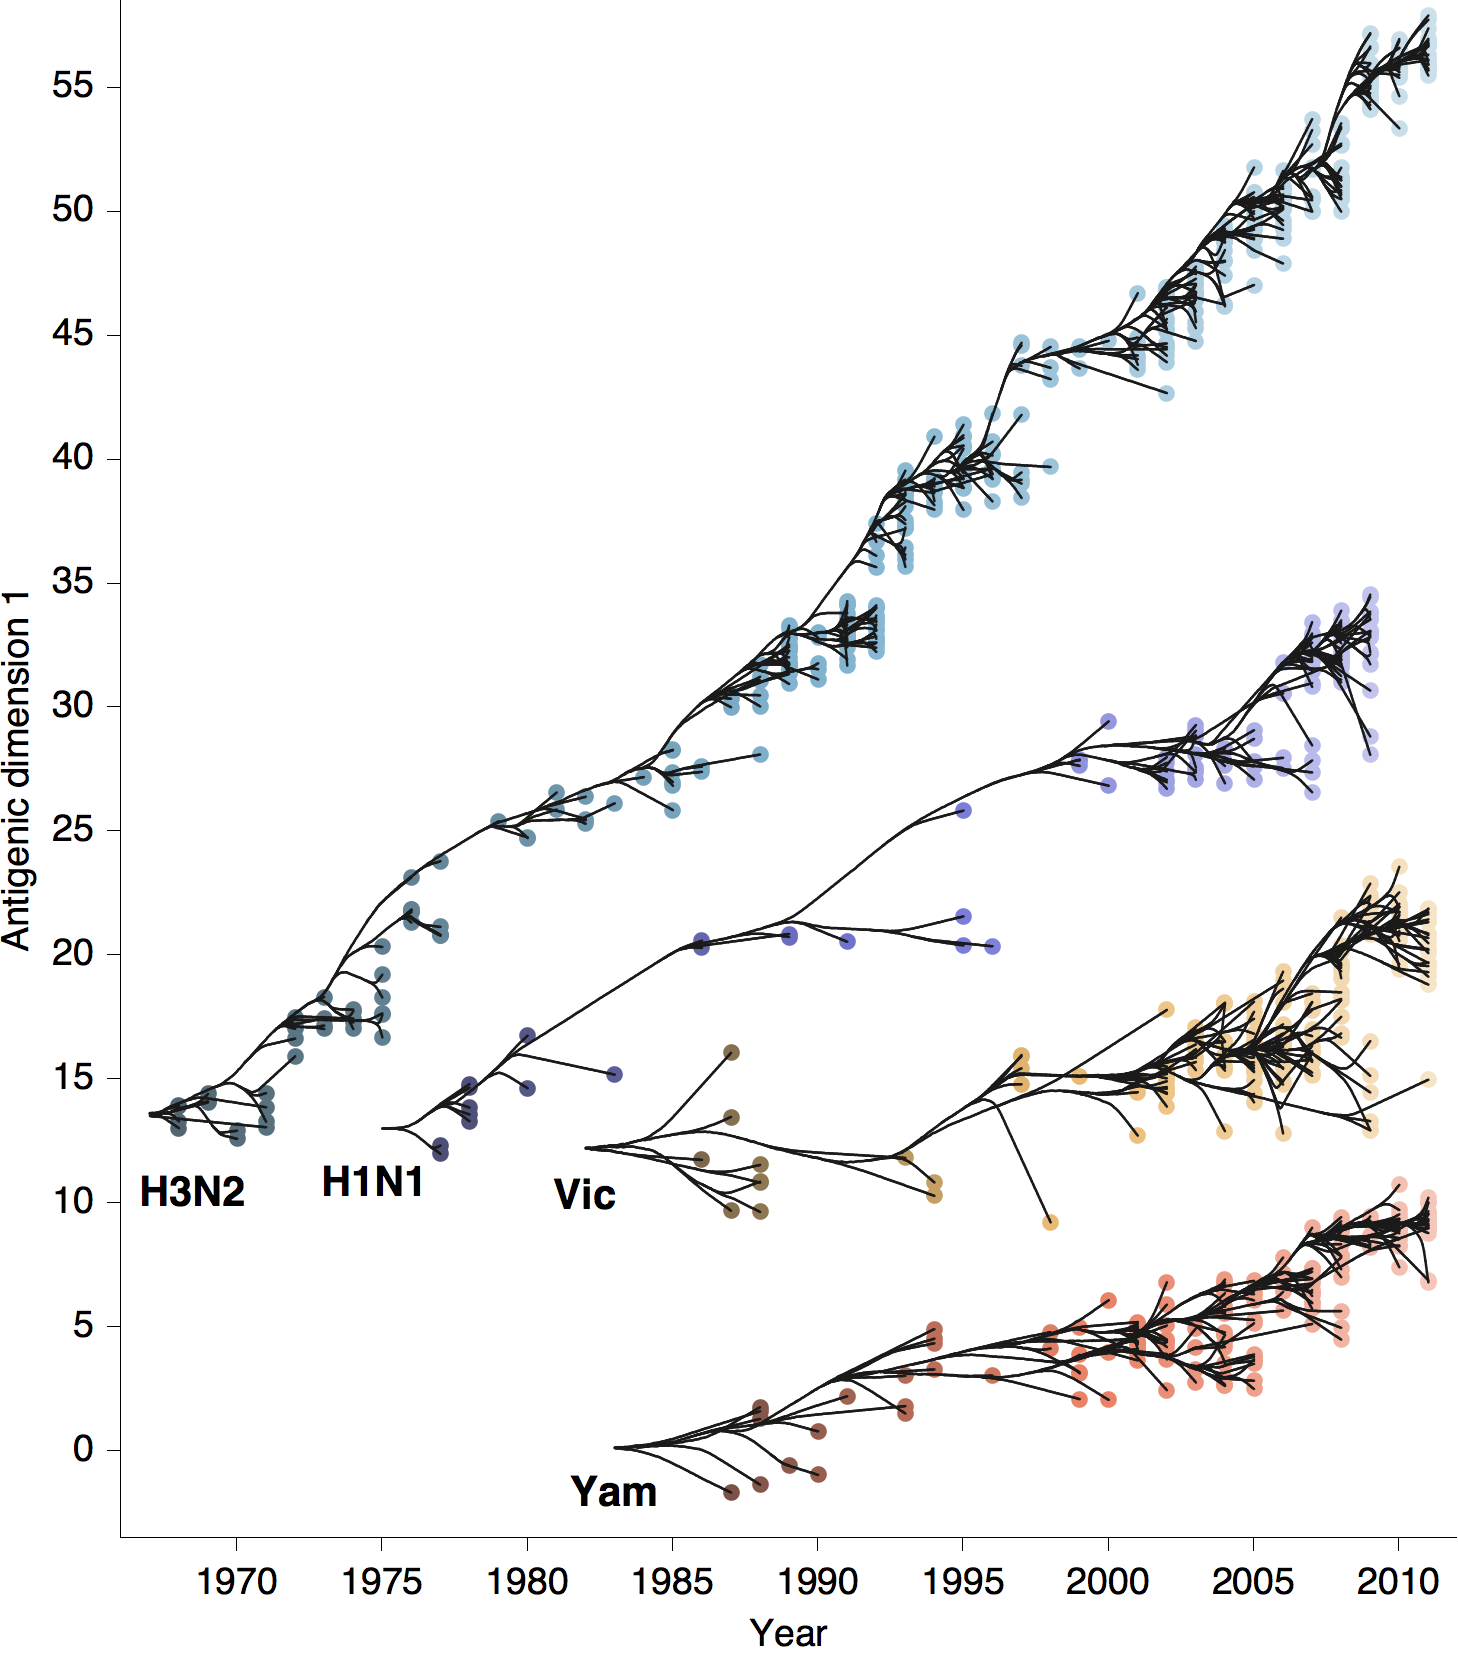
\includegraphics[width=0.75\textwidth]{figures/drift}
	\caption{\textbf{Antigenic drift of A/H3N2, A/H1N1, B/Vic and B/Yam viruses showing evolutionary relationships between virus samples.} 
	Antigenic drift is shown in terms of change of location in the first antigenic dimension through time.
	Circles represent a posterior sample of virus locations and have been shaded based on year of isolation.
	Antigenic units represent two-fold dilutions of the HI assay.
	Distances between clades, e.g.\ A/H3N2 and A/H1N1, are arbitrary.
	Lines represent mean posterior diffusion paths when virus locations are fixed.} 
	\label{drift} 
\end{figure}

We find that other clades of influenza evolved in antigenic phenotype substantially slower than A/H3N2 (Figure~\ref{drift}).
Influenza A/H1N1 evolved at a rate of 0.62 units per year (HPD 0.56--0.67), but showing a similar pattern of punctuated antigenic evolution with occasional larger jumps in phenotype, such as the emergence of the Solomon Islands/06 cluster.  
Influenza B/Victoria also evolved relatively slowly, with an average rates of 0.42 (HPD 0.32--0.51) units per year.
Influenza B/Vic appears to show some degree of punctuated antigenic evolution with a recent transition creating the Brisbane/08 cluster.
Interestingly, a minor lineage of B/Vic has persisted through 2011, appearing antigenically distinct from other 2011 viruses (Figure~\ref{drift}), though the eventual fate of this lineage has yet to be determined.
Influenza B/Yamagata evolved slower still, with an average rate of and 0.32 (HPD 0.25--0.39) units per year.
Little punctuated evolution is obvious in the evolution of B/Yam.

Interestingly, although antigenic clusters seem to emerge in a punctuated fashion in influenza A/H3N2, year-to-year antigenic drift relatively constant through time with most years exhibiting an intermediate level of drift (Figure~\ref{jumps}).
We calculate year-to-year antigenic drift for years 1992 to 2011 by calculating the average location along dimension 1 of phylogenetic lineages present at year $i$ and comparing this location to the average location of phylogenetic lineages present at year $i-1$.
For A/H3N2, the largest cluster transition we observe is the emergence of the Sydney/97 cluster, evident as the appearance in 1997 of a large gap in virus locations along antigenic dimension 1 (Figure~\ref{drift}).
However, in 1997 only three of the nine viruses sampled show the Sydney/97 phenotype, while the remaining six viruses exhibit the old Wuhan/95 phenotype.
In 1998, three of the four viruses sampled show the Sydney/97 phenotype, with the remaining virus still showing the Wuhan/95 phenotype.
In 1999, all sampled viruses exhibit the Sydney/97 phenotype.
Thus, we observe fairly equal rates of year-to-year antigenic drift in mean phenotype in going from 1996 to 1997, from 1997 to 1998 and from 1998 to 1999, rather than all drift in mean antigenic phenotype attributable to a shift in 1997 (Figure~\ref{jumps}).
In addition to showing greater overall rates of antigenic drift, A/H3N2 shows greater variation in year-to-year drift than seen in A/H1N1 or influenza B (Figure~\ref{jumps}).
We find that the standard deviation in year-to-year drift is 0.88 antigenic units for A/H3N2, 0.51 units for A/H1N1, 0.54 units for B/Vic and 0.27 units for B/Yam.

%%% jumps %%%
\begin{figure}[h]
	\centering		
	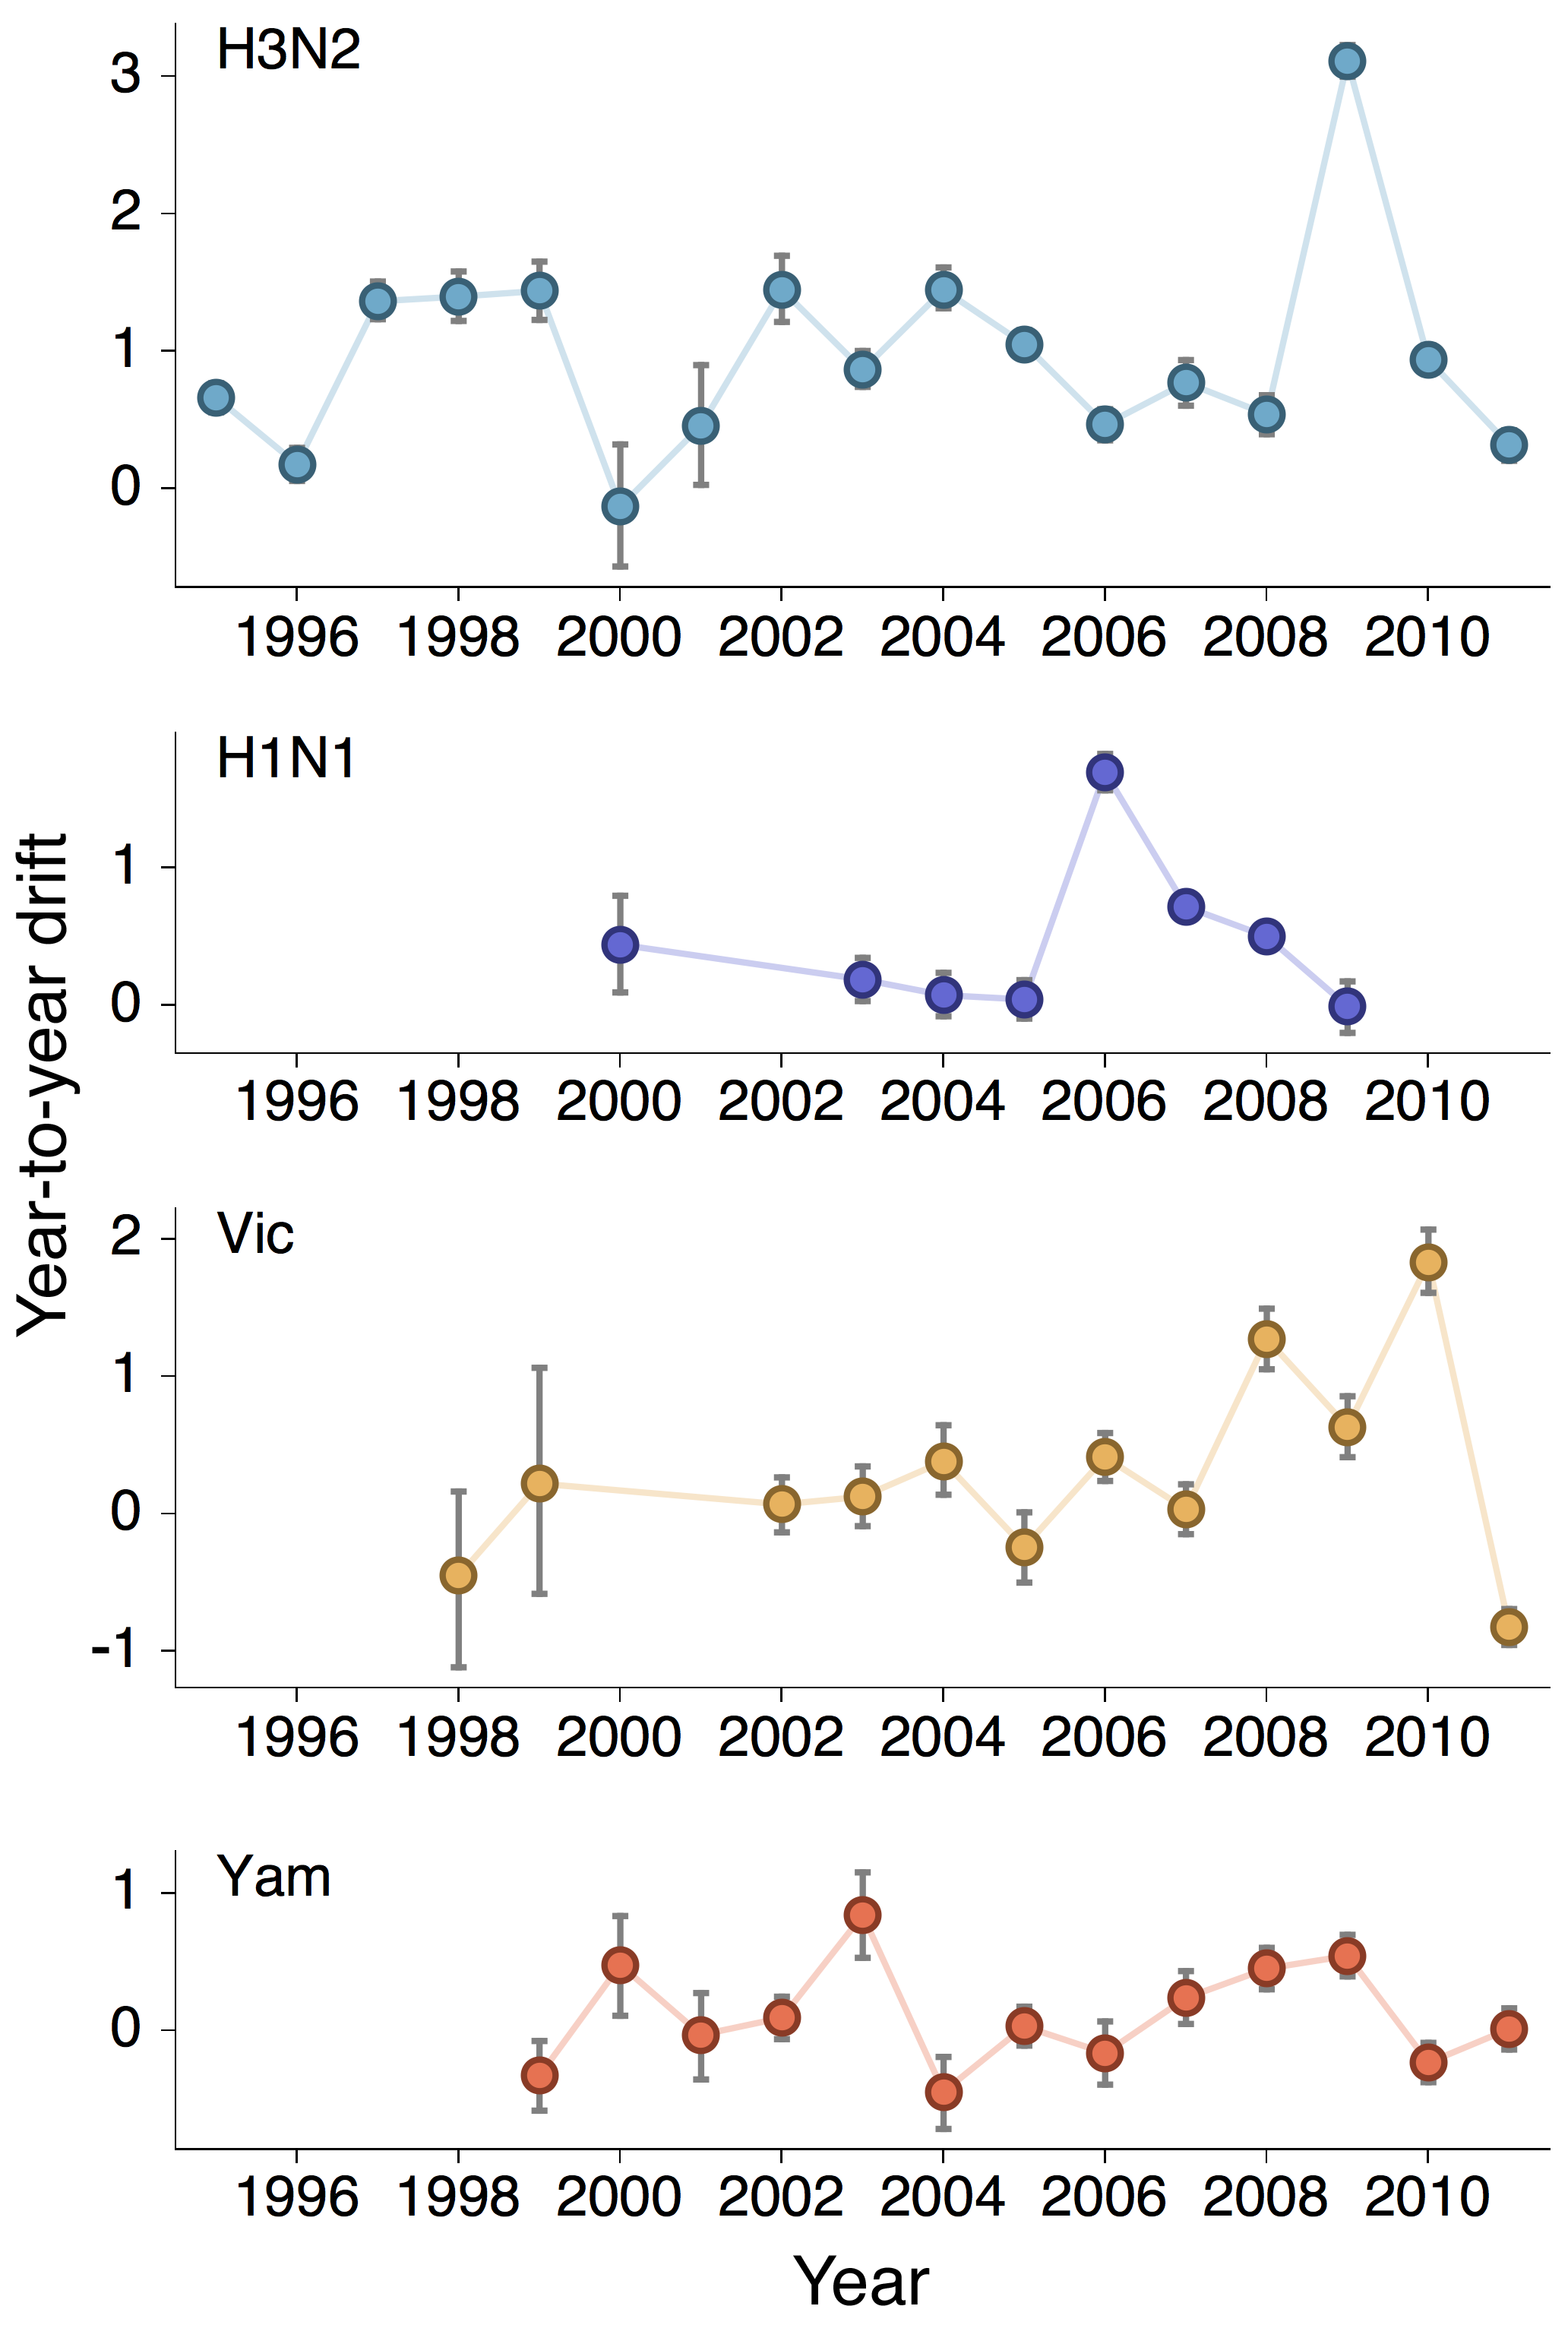
\includegraphics[width=0.95\textwidth]{figures/jumps}
	\caption{\textbf{Year-to-year antigenic drift between 1992 and 2011 in A/H3N2, A/H1N1, B/Vic and B/Yam viruses.} 
	(A) Timeseries of year-to-year antigenic drift across influenza clades from 1992 to 2011.
	Year-to-year antigenic drift for a virus clade for year $i$ is measured as the mean of antigenic dimension 1 of phylogenetic lineages in year $i$ compared to the mean of antigenic dimension 1 of phylogenetic lineages from the previous year $i-1$.
	For example, 2000 represents difference in antigenic dimension 1 between 1999 and 2000.
	Error bars represent 50\% credible intervals across posterior samples of year-to-year drift.
	(B) Histograms of year-to-year antigenic drift across influenza clades summarizing observations from 1992 to 2011.
	} 
	\label{jumps} 
\end{figure}

\subsection*{Epidemiological consequences of antigenic drift}

We investigated the relative rates of antigenic evolution in A/H3N2, A/H1N1, B/Vic and B/Yam from 2000 to 2011, finding a general correspondence between antigenic drift in dimension 1 and relative incidence within each influenza clade (Figure~\ref{incidence}).
Here, we take the measurements of year-to-year antigenic drift from the preceding section (Figure~\ref{jumps}) and calculate the relative contribution to total antigenic drift for each clade in each year.
We compare these measurements of relative antigenic drift to relative isolations of viruses from each clade in the USA from the 2001--2002 to the 2011--2012 influenza seasons (see Methods).
From 2000 to 2011, A/H3N2 accounted for the majority of antigenic drift (46\%), while A/H1N1, B/Vic and B/Yam split the remainder, accounting for 18\%, 21\% and 15\%, respectively.
Similarly, A/H3N2 was responsible for the majority of incidence (58\%) during this time period.
Influenza A/H1N1 accounted for 18\% of incidence, B/Vic accounted for 16\% of incidence and B/Yam accounted for 7\% of incidence.
These proportions are significantly similar to one another (randomization test, $p = 0.030$).

%%% incidence %%%
\begin{figure}[tb]
	\centering		
	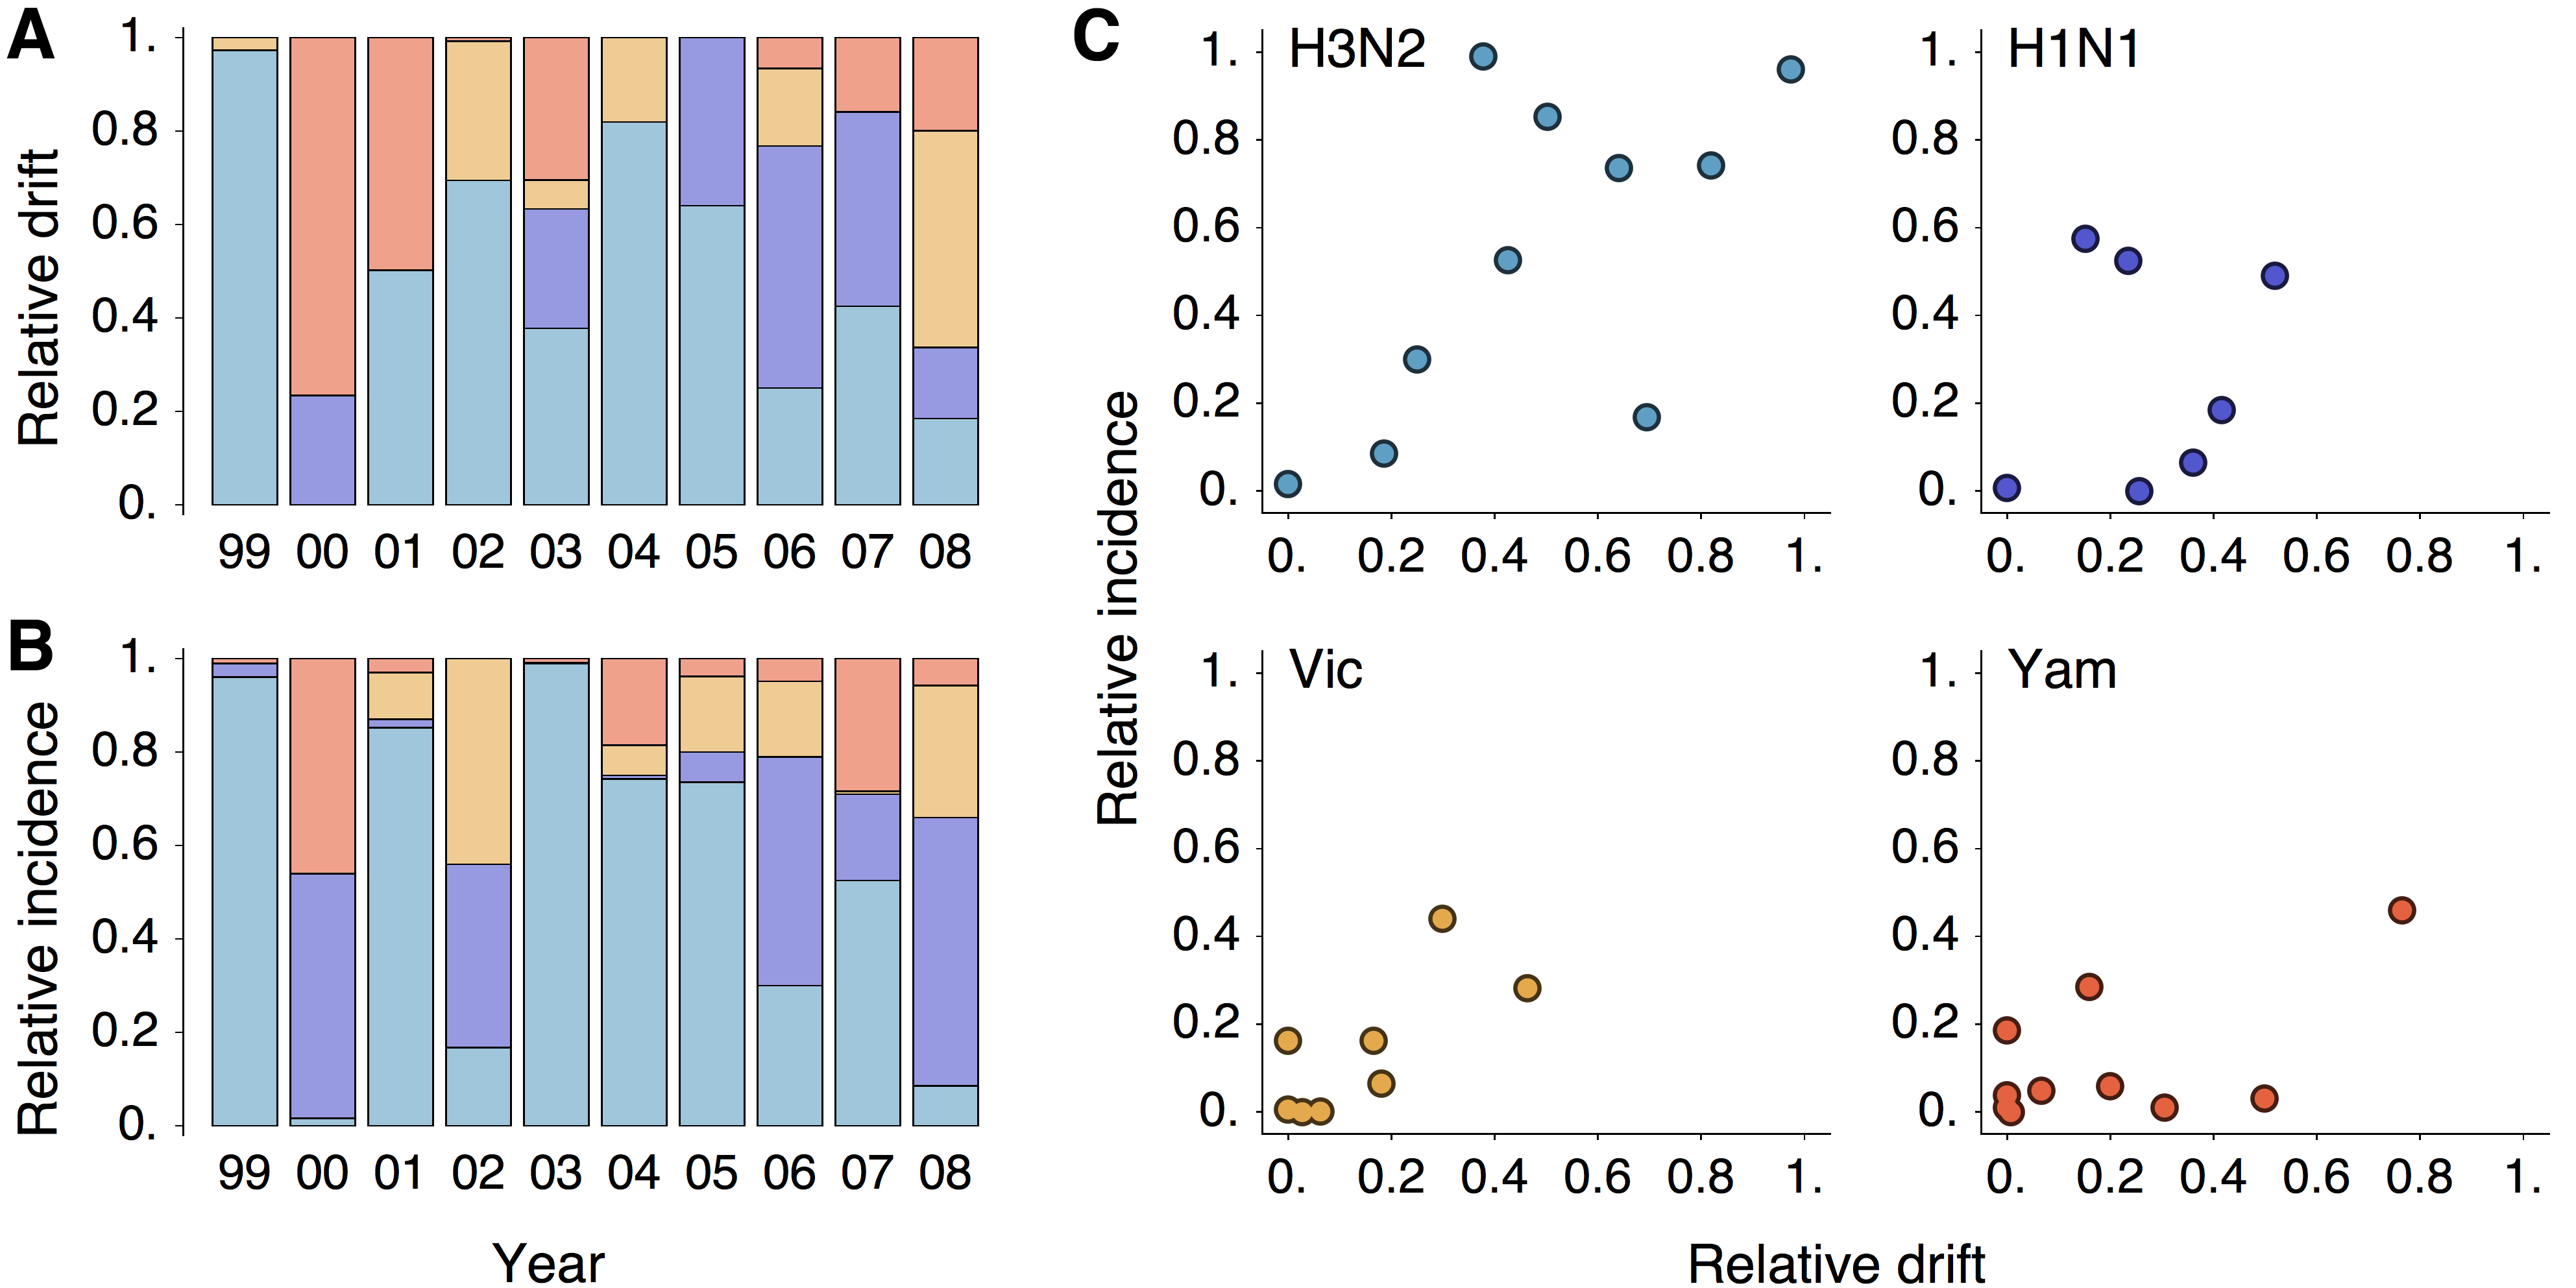
\includegraphics[width=0.9\textwidth]{figures/incidence}
	\caption{\textbf{Relative antigenic drift and relative incidence of A/H3N2, A/H1N1, B/Vic and B/Yam from 2000 to 2011.} 
	(A) Relative antigenic drift of influenza clades.
	Relative antigenic drift for A/H3N2 is measured as the drift of A/H3N2 viruses divided by the sum of drift for A/H3N2, A/H1N1, B/Vic and B/Yam.
	For example, `01' signifies difference in antigenic dimension 1 between 2000 and 2001.
	Years with negative absolute drift were assigned a relative antigenic drift of 0.
	(B) Relative incidence of influenza clades determined through relative isolation counts in the USA for winter influenza seasons.
	Here, `01' refers to the 2001/2002 influenza season.
	(C) Correlation of relative antigenic drift and relative incidence in each influenza clade.
	Scatterplots represent drift from year $i-1$ to year $i$ compared to incidence in winter season beginning in year $i$, e.g. drift from 2000 to 2001 compared to incidence in the 2001/2002 influenza season.
	} 
	\label{incidence} 
\end{figure}

Additionally, year-to-year comparisons show a similar pattern, in which years with high levels of antigenic drift coming into an influenza season, e.g.\ drift from 2000 to 2001, show high levels of relative incidence in that season, e.g.\ incidence in the 2001/2002 season (Figure~\ref{incidence}). 
We find an overall correlation between clade-specific relative antigenic drift and clade-specific incidence of $r = 0.71$ (Pearson correlation, $p = 6.43 \times 10^{-8}$).
Correlation is present to greater of lesser degrees for each of the four clades, with $r_\mathrm{H3} = 0.56$, $r_\mathrm{H1} = 0.46$, $r_\mathrm{Vic} = 0.49$ and $r_\mathrm{Yam} = 0.23$.
Pandemic H1N1 is present in the incidence data in 2009 and afterwards, however, our estimates of relative incidence only include isolations of seasonal A/H3N2, A/H1N1, B/Vic and B/Yam.

These findings clearly demonstrate the epidemiological importance of antigenic drift and show that incidence of influenza clades A/H3N2, A/H1N1, B/Vic and B/Yam is strongly impacted by levels of antigenic drift within each clade.
Furthermore, these findings suggest that the composition of a particular influenza season could be estimated ahead of time by examining the degree of antigenic drift between influenza clades.
However, these findings alone do not conclusively show interference between clades; more work needs to be done to establish whether antigenic drift within one influenza clades drives down incidence in other clades.

\subsection*{Conversion of antigenic mutation into fixed differences}

We observe a faster rate of antigenic drift in influenza A/H3N2 than in A/H1N1 or in either lineage of influenza B.
Previous work using general epidemiological models has suggested that rates of antigenic drift may be influenced by both fundamental reproductive number $R_0$ and rate cross-immunity decreasing mutation \cite{Gog02,Lin03}.
Owing to these and similar findings, subsequent work ascribed differences in the evolution of A/H3N2 relative to A/H1N1 and influenza B to either greater $R_0$ or greater mutation rate \cite{Ferguson03,Bedford12}.
Here, we examine the conversion of recently acquired antigenic mutation into fixed differences by comparing rates of antigenic diffusion to the degree of persistence on phylogeny branches in A/H3N2, A/H1N1, B/Vic and B/Yam (Table~\ref{diffusiontable}).
To facilitate comparisons, we measure the diffusion coefficient $D$ \cite{Pybus12} characterizing the antigenic movement of each influenza lineage (see Supp.\ Methods).
This coefficient is measured in terms of units$^2$/year and can be used to determine the diffusion length scale, that is the expected relationship between time and distance traveled, which is $2 \sqrt{t D}$ for a two-dimensional diffusion.
Higher diffusion coefficients mean a lineage is diffusing faster through antigenic space.
We compare diffusion coefficients between trunk branches and side branches, where trunk branches are defined as branches ancestral to the most recent virus sample and side branches are defined as those branches not ancestral to the most recent virus sample.

%%% diffusiontable %%%
\begin{table}[h]
	\centering
	\caption{\textbf{Estimates of fundamental diffusion coefficient $D$ across influenza lineages and phylogenetic branches, including posterior means and 50\% highest posterior density intervals.}}
	\label{diffusiontable}	
	\begin{tabular}{ c c c c } 
	\hline
	Lineage	&	Trunk branch $D$ 	& 	Side branch $D$		& 	Ratio \\
	\hline		
	A/H3N2	&	0.90 (0.79--0.97)	&	0.62 (0.57--0.65)	&	1.45 (1.31--1.57) \\
	A/H1N1	&	0.62 (0.50--0.71)	&	0.44 (0.38--0.48)	&	1.45 (1.18--1.70) \\
	B/Vic	&	0.63 (0.51--0.71)	&	0.62 (0.54--0.68)	&	1.02 (0.87--1.14) \\
	B/Yam	&	0.35 (0.29--0.40)	&	0.33 (0.28--0.36)	&	1.09 (0.93--1.23) \\
	\hline
	\end{tabular}	
\end{table}

Mutations must proceed through the sieve of natural selection, first appearing as transient differences restricted to side branches, while advantageous mutations will preferentially fix in the virus population and thus accrue on the trunk of the phylogeny.
We expect the diffusion coefficient on side branches to more closely resemble the raw rate of antigenic mutation.
Here, we find that A/H3N2 and B/Vic have similar diffusion coefficients, which are larger than the diffusion coefficients of A/H1N1 and B/Yam (Table~\ref{diffusiontable}).
Thus, we expect that new antigenic mutations may occur at a faster rate in A/H3N2 and B/Vic than in A/H1N1 or B/Yam.
We find that trunk branches in both A/H3N2 and A/H1N1 evolve in antigenic phenotype faster than side branches (Table~\ref{diffusiontable}), suggesting that positive selection is promoting antigenic movement in these lineages.
Interestingly, B/Vic and B/Yam show less of a signature of positive selection, with similar diffusion coefficients on trunk and side branches (Table~\ref{diffusiontable}).
Thus, although drift forward along dimension 1 is promoted in all lineages (Figure~\ref{drift}), raw antigenic diffusion appears to be promoted more strongly in influenza A than in influenza B, giving an advantage to influenza A in terms of overall rate of antigenic drift.
Additionally, it appears that A/H3N2 and B/Vic benefit from a greater influx of new antigenic mutations, giving them an advantage over their sister lineages A/H1N1 and B/Yam also in terms of overall rate of antigenic drift.

In this context, it is especially interesting that adaptive evolution in the HA1 protein determined through analysis of nonsynonymous and synonymous substitutions is substantially stronger in A/H3N2 than in A/H1N1 \cite{Wolf06}; H3 appears to accumulate adaptive fixations at $\sim$150\% the rate of H1 \cite{Bhatt11}.
Here, we observe that A/H3N2 has a diffusion coefficient $\sim$141\% greater than A/H1N1 along side branches of the phylogeny.
These results suggest that the greater rate of adaptive fixation in A/H3N2 may be simply due to a greater abundance of new antigenic mutations to fix.

We suggest that the larger signal of positive selection for antigenic diffusion in influenza A relative to influenza B could be due to either a greater fundamental reproductive number $R_0$ or to pleiotropic effects associated with antigenic change.
In the later case, we expect that many antigenic variants may be at inherent disadvantage against other strains from decreased protein function \cite{Kaverin04,Rudneva12} or other effects, even though they benefit from a transmission advantage mediated by host immunity.
These mutations may not be promoted by natural selection to the same extent as antigenic variants that maintain functional equivalence.
Still, it is clear that more work is necessary to fully clarify the the mechanistic underpinnings of the relative evolutionary success of different influenza lineages.

%%% CONCLUSIONS %%%
\section*{Conclusions}

In this study we provide a foundation for evolutionary antigenic cartography, which seeks to simultaneously assess antigenic phenotype and antigenic evolution.
We use this approach to characterize competitive dynamics across influenza clades A/H3N2, A/H1N1, B/Vic and B/Yam and show that antigenic evolution drives strain replacement in each influenza clade.
We find that varying levels of mutational input and varying efficiencies of the conversion of antigenic polymorphism into fixed differences results in different rates of antigenic drift across influenza clades.
Influenza A/H3N2 benefits from a higher rate of new antigenic mutation coupled with strong adaptive evolution and evolves in antigenic phenotype faster than A/H1N1, B/Vic and B/Yam.
Correspondingly, we observe substantially greater levels of incidence in A/H3N2 than in other influenza clades.
We suggest that antigenic evolution strongly influences competitive dynamics both within and between influenza clades.

The statistical framework presented here represents a baseline to which further advancements in modeling antigenic phenotype and evolution may be made.
For example, our likelihood-based model facilities the inclusion of possible covariates affecting immunological titer, which could include experimental factors such as red blood cell type used in the HI assay \cite{Lin12} and whether oseltamivir is included in the HI reaction \cite{Lin10}.
Additionally, this framework should be ideally suited to uncovering genetic determinants of antigenic change, as both the sequence state and antigenic location of internal nodes in the phylogeny may be estimated.
In this fashion, it should be possible to correlate sequence substitutions directly to antigenic diffusion.

Further work characterizing antigenic evolution in the human influenza virus may eventually prove to be crucial in improving vaccine strain selection.

%%% METHODS %%%
\section*{Methods}

\subsection*{Antigenic cartography}

Antigenic characteristics of viral strains are often assessed through immunological assays such as the hemagglutination inhibition (HI) assay \cite{Hirst43}.  
At heart, these assays compare the reactivity of one virus strain to antibodies raised against another virus strain via challenge or vaccination.  
In the case of HI, the measurement of cross-reactivity takes the form of a titer representing the dilution factor at which serum raised against a particular virus ceases to be effective at inhibiting binding to red blood cells of another virus.  
These factors are commonly assessed by serial dilution, so that HI titers will form a log series, 40, 80, 160, etc \dots.
Because experimental HI titers typically differ by factors of two, we find it convenient to work in log$_2$ space and represent the titer of virus $i$ against serum $j$ as $H_{ij} = \mathrm{log}_2 \mbox{(HI titer)}$, i.e.\ a titer of 160 has $H_{ij} = 7.32$.
Due to experimental constraints, most comparisons cannot be made, leading to a sparse observation matrix $\mathbf{H} = \{H_{ij}\}$.  
Further, measurements are usually interval and truncated, e.g.\ inhibition may cease somewhere between the serial titers of 160 and 320, or inhibition may be absent at all titers assayed, suggesting a threshold somewhere between 0 and 40.  

Previous work \cite{Smith04, Cai10} has used multidimensional scaling to place viruses and sera on an `antigenic map'.  
These methods heuristically optimize locations of viruses and sera by seeking to minimize the sum of squared errors between titers predicted by map locations and observed titers.  
Antigenic maps produced by these methods have proved useful in categorizing virus phenotypes \cite{Smith04}, but the extension of these methods to integrate genetic data remains notably lacking.

Here, we follow previous models in representing antigenic locations as points in a low $P$-dimensional antigenic map. 
One of our initial goals is to find an optimal projection of the high-dimensional distance matrix $\mathbf{H}$ into this lower dimensional space. 
We conduct this projection using Bayesian multidimensional scaling (BMDS) \cite{Oh01} in which we construct a probabilistic model to quantify the fit of a particular configuration of cartographic locations to the observed matrix of serological measurements.
Typically, $P = 2$, but higher or lower dimensions may better reflect the data. 

\subsection*{Likelihood functions}

Let $\virus_i \in \mathbb{R}^{P}$ represent the cartographic location of virus $i$ for $i = 1,\ldots,\vn$, so that $\virus_i = (x_{i1}, x_{i2})^{\prime}$ for $P=2$. 
Similarly, let $\serum_j$ represent the cartographic location of serum $j$ for $j = 1,\ldots,\sn$, so that $\serum_j = (y_{j1},y_{j2})^{\prime}$ for $P=2$.
For notational compactness, we collect together all virus coordinates into an $\vn \times P$ matrix  $\viruses = (\virus_1, \ldots, \virus_{\vn})^{\prime}$ and all serum coordinates into an $\sn \times P$ matrix $\sera = (\serum_{1},\ldots,\serum_{\sn})^{\prime}$.
Virus and serum may be isolated from / raised against the same strain and have different cartographic locations, and separate serum isolates raised against the same strain may also have different cartographic locations. 
This gives a set of distances between virus and serum cartographic locations 
\begin{equation}
	\delta_{ij} =  || \virus_i - \serum_j ||_2,
\end{equation}
where $|| \cdot ||_2$ is an $L_2$ norm.

Traditional approaches to antigenic cartography \cite{Smith04} begin by defining immunological distance as
\begin{equation}
	d_{ij} =  \se_j - H_{ij},
\end{equation}
where $H_{ij}$ is the log$_2$ titer of virus $i$ against serum $j$ and serum effect $\se_j = \max ( H_{1j},\ldots,H_{\vn j} )$ is fixed.
In following multidimensional scaling (MDS), these approaches attempt to optimize over unknown $\viruses$ and $\sera$ such that
\begin{equation}
	\sum_{(i,j) \in \cal I} 
	\left(
		\delta_{ij} - d_{ij}
	\right)^2
\end{equation}
is minimized, where $\mathcal{I} = \{ (i,j) : H_{ij} \mbox{ is measured} \}$.

Here, we instead assume a probabilistic interpretation in which an observed titer is normally distributed around its cartographic expectation with variance $\mdssd^2$,
\begin{equation} \label{hij}
	H_{ij} \sim \normal( \se_j - \delta_{ij}, \, \mdssd^2 ).
\end{equation}
Consequently, the likelihood of observing an exact titer given the placement of antigenic locations is 
\begin{equation} 
	\point(H_{ij}) = \phi \left( \frac{ H_{ij} + \delta_{ij} - \se_j }{ \mdssd } \right),
\end{equation}
where $\phi(\cdot)$ represents the standard normal probability density function (PDF).
Previous BMDS has employed a sampling density truncated to strictly positive quantities since $d_{ij}$ are directly observed, non-negative quantities.  
In the antigenic setting, these remain random and can be negative since neither $\se_j$ is known nor is $H_{ij}$ observed with much precision. 

HI assays sometimes show no inhibition at all measured titrations, e.g.\ a measurement can be reported as `$<$40'.
In this case, the likelihood of observing the threshold measurement follows the cumulative density of the lower tail of the normal distribution
\begin{equation} 
	\threshold(H_{ij}) = \Phi \left( \frac{ H_{ij} + \delta_{ij} - \se_j }{ \mdssd } \right),
\end{equation}
where $\Phi(\cdot)$ represents the standard normal cumulative distribution function (CDF).
Although it is simplest to assume that immunological measurements represent point estimates, it seems more natural to assume that the threshold for inhibition occurs between two titers, e.g.\ we observe inhibition at 1:160 dilution and no inhibition at 1:320 dilution.
Rather than taking the HI titer as 160, we can instead treat this as an interval measurement, assuming that the exact titer for inhibition would occur somewhere between 160 and 320.
HI titers are usually reported as the highest titer that successfully inhibits virus binding, so that in this case, we calculate the likelihood of an interval measurement as
\begin{equation} 
	\interval(H_{ij}) = \Phi \left( \frac{ H_{ij} + \delta_{ij} - \se_j + 1 }{ \mdssd } \right) - \Phi \left( \frac{ H_{ij} + \delta_{ij} - \se_j }{\mdssd} \right).
\end{equation}
These likelihoods are illustrated in Figure~\ref{hij_likelihood}.
Throughout our analyses, we use interval likelihoods $\interval$ rather than point likelihoods $\point$ unless otherwise noted.

%%% hij_likelihood %%%
\begin{figure}[tb]
	\centering		
	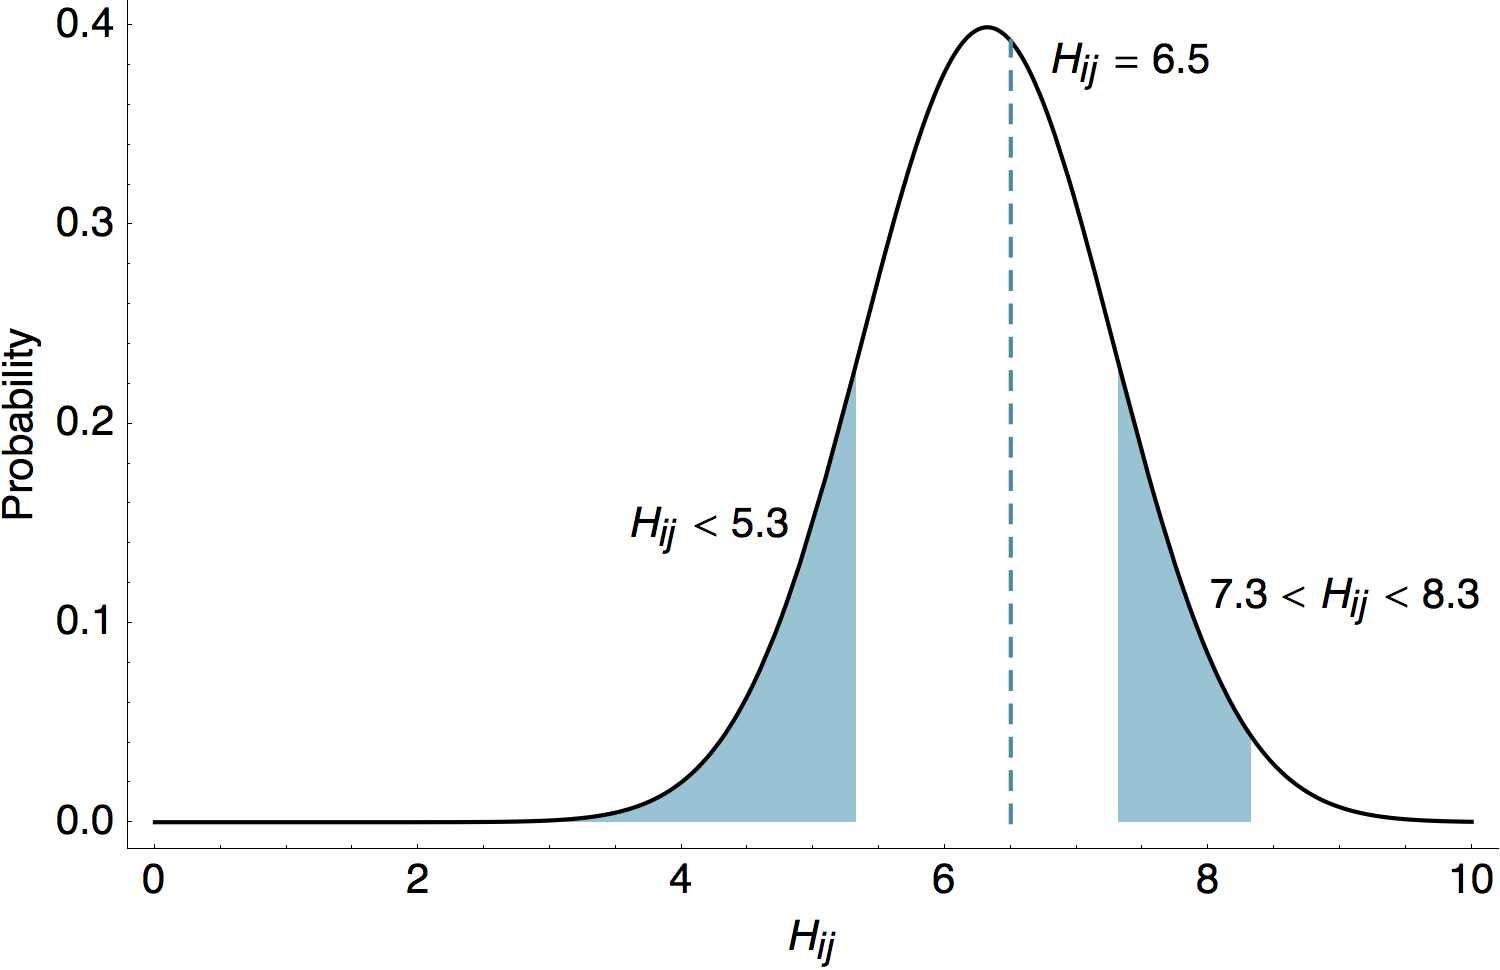
\includegraphics[width=0.6\textwidth]{figures/hij_likelihood}
	\caption{\textbf{Likelihood of HI titers in the BMDS model.} 
	Here we show the likelihoods of observing three different outcomes given $\delta_{ij} = 4$, $\mdssd = 0.95$ and $\se_j = \mathrm{log}_2 (1280) = 10.32$.  
	The likelihood of observing a threshold titer of `$<$40' is equal to the lower tail of the probability density function $\threshold(5.32) = 0.146$.
	The likelihood of observing a point measurement with an exact inhibiting titer of `90.5' is equal to the density function $\point(6.5) = 0.413$.
	The likelihood of observing an interval measurement with an inhibiting titer somewhere between `160' and `320' is equal to $\interval(7.32) = 0.129.$
	} 
	\label{hij_likelihood} 
\end{figure}

We calculate the overall likelihood by multiplying probabilities of individual measurements
\begin{equation} 
	L(\viruses,\sera) = \prod_{(i,j) \in \cal I} f(H_{ij}),
\end{equation}
using probability functions $\point$, $\threshold$ and $\interval$ as appropriate.
We begin by assuming independent, diffuse normal prior on virus and serum locations
\begin{eqnarray}
	\virus_i &\sim& \mathrm{Normal}(\boldsymbol{\mu},\boldsymbol{\Sigma}) \nonumber \\
	\serum_j &\sim& \mathrm{Normal}(\boldsymbol{\mu},\boldsymbol{\Sigma}),
\end{eqnarray}
with $\boldsymbol{\mu} = (0,\ldots,0)^{\prime}$ and $\boldsymbol{\Sigma}$ is a diagonal matrix with diagonal elements all equal to $10000$.

\subsection*{Virus and serum effects}

The preceding model represents immunological distance as a drop in titer against the most reactive comparison for a particular serum.
However, this model may be biased in some circumstances.
In one example, if a particular serum $j$ is only measured against distant viruses, its maximum titer will be artificially low and the likelihoods concerning this serum will appear poor. 
To address this issue, we relax the assumption of fixed $\se_j$ values and treat the expected log$_2$ titer when $\delta_{ij}=0$ as a random variable.
In this case, $H_{ij}$ still follows equation \ref{hij} with expectation $\se_j - \delta_{ij}$, but the vector of `serum effects' $\ses = (\se_1,\ldots,\se_{\sn})$ is random and estimated rather than fixed.
We assume that $\se_j$ values are hierarchically distributed according to a normal distribution.   
We take an Empirical Bayesian approach in specifying the mean and variance of this distribution, set to the empirical mean and empirical variance of the set of maximum titers across sera $\{ \max ( H_{1j},\ldots,H_{\vn j} ) : j = 1,\ldots,\sn \}$.
This formulation assumes that particular sera are more reactive in general than other sera.

Additionally, we follow the same logic and assume that some virus isolates are more reactive than other virus isolates and include a `virus effect' $\ve_i$ representing the general level of reactivity across HI assays. 
With virus reactivity included, observed titers follow
\begin{equation}
	H_{ij} \sim \normal \left( \frac{\ve_i+\se_j}{2} - \delta_{ij}, \, \mdssd^2 \right),
\end{equation}
and the vector of virus effects $\ve_i$ for $i = 1,\ldots, \vn$ is estimated in an analogous hierarchical fashion, with $\ves$ normally distributed with mean and variance equal to the empirical mean and variance of the set of maximum titers across viruses $\{ \max ( H_{i1},\ldots,H_{i \sn} ) : i = 1,\ldots,\vn \}$.

\subsection*{Location prior}

As presented, virus and serum locations $\viruses$ and $\sera$ give a likelihood of observing the HI data $\mathbf{H}$.
However, distances between viruses and sera represent only a local description of antigenic space and do not provide a global picture.
An example of this phenomenon is shown in Figure~\ref{schematic_map}.
In this case it is impossible to determine from the HI data at hand whether the blue and yellow viruses are antigenically similar or antigenically divergent. 
This presents an issue of model identifiability; multiple antigenic maps give the same likelihood of observing the serological data.
In order to achieve more interpretable antigenic locations we impose a weak prior on global locations.
In influenza, it's clear that antigenic distance between strains increases with time \cite{Smith04,Cai10}.
To capture this, we replace our previous diffuse prior with an informed prior in which the expected location of viruses and sera increases with date of sampling along dimension one, and each virus and serum location follows an independent normal distribution centered around this temporal expectation, so that
\begin{eqnarray}
	x_{i1} &\sim& \beta \, t_i + \normal(0, \virussd^2) \nonumber \\
	y_{j1} &\sim& \beta \, t_j + \normal(0, \serumsd^2),
\end{eqnarray}
where $t$ is the difference between the date of the indexed virus or serum and the date of the earliest sampled virus or serum, and other dimensions follow $x_{im} \sim \normal(0, \virussd^2)$ and $y_{jm} \sim \normal(0, \serumsd^2)$ for $m\ge2$.
Thus, this model assumes that virus and serum locations drift in a line across the antigenic map at rate $\beta$.
The parameter $\virussd$ determines the breadth of the cloud of virus locations at each point in time, while $\serumsd$ determines the breadth of the cloud of serum locations.

%%% schematic_map %%%
\begin{figure}[tb]
	\centering		
	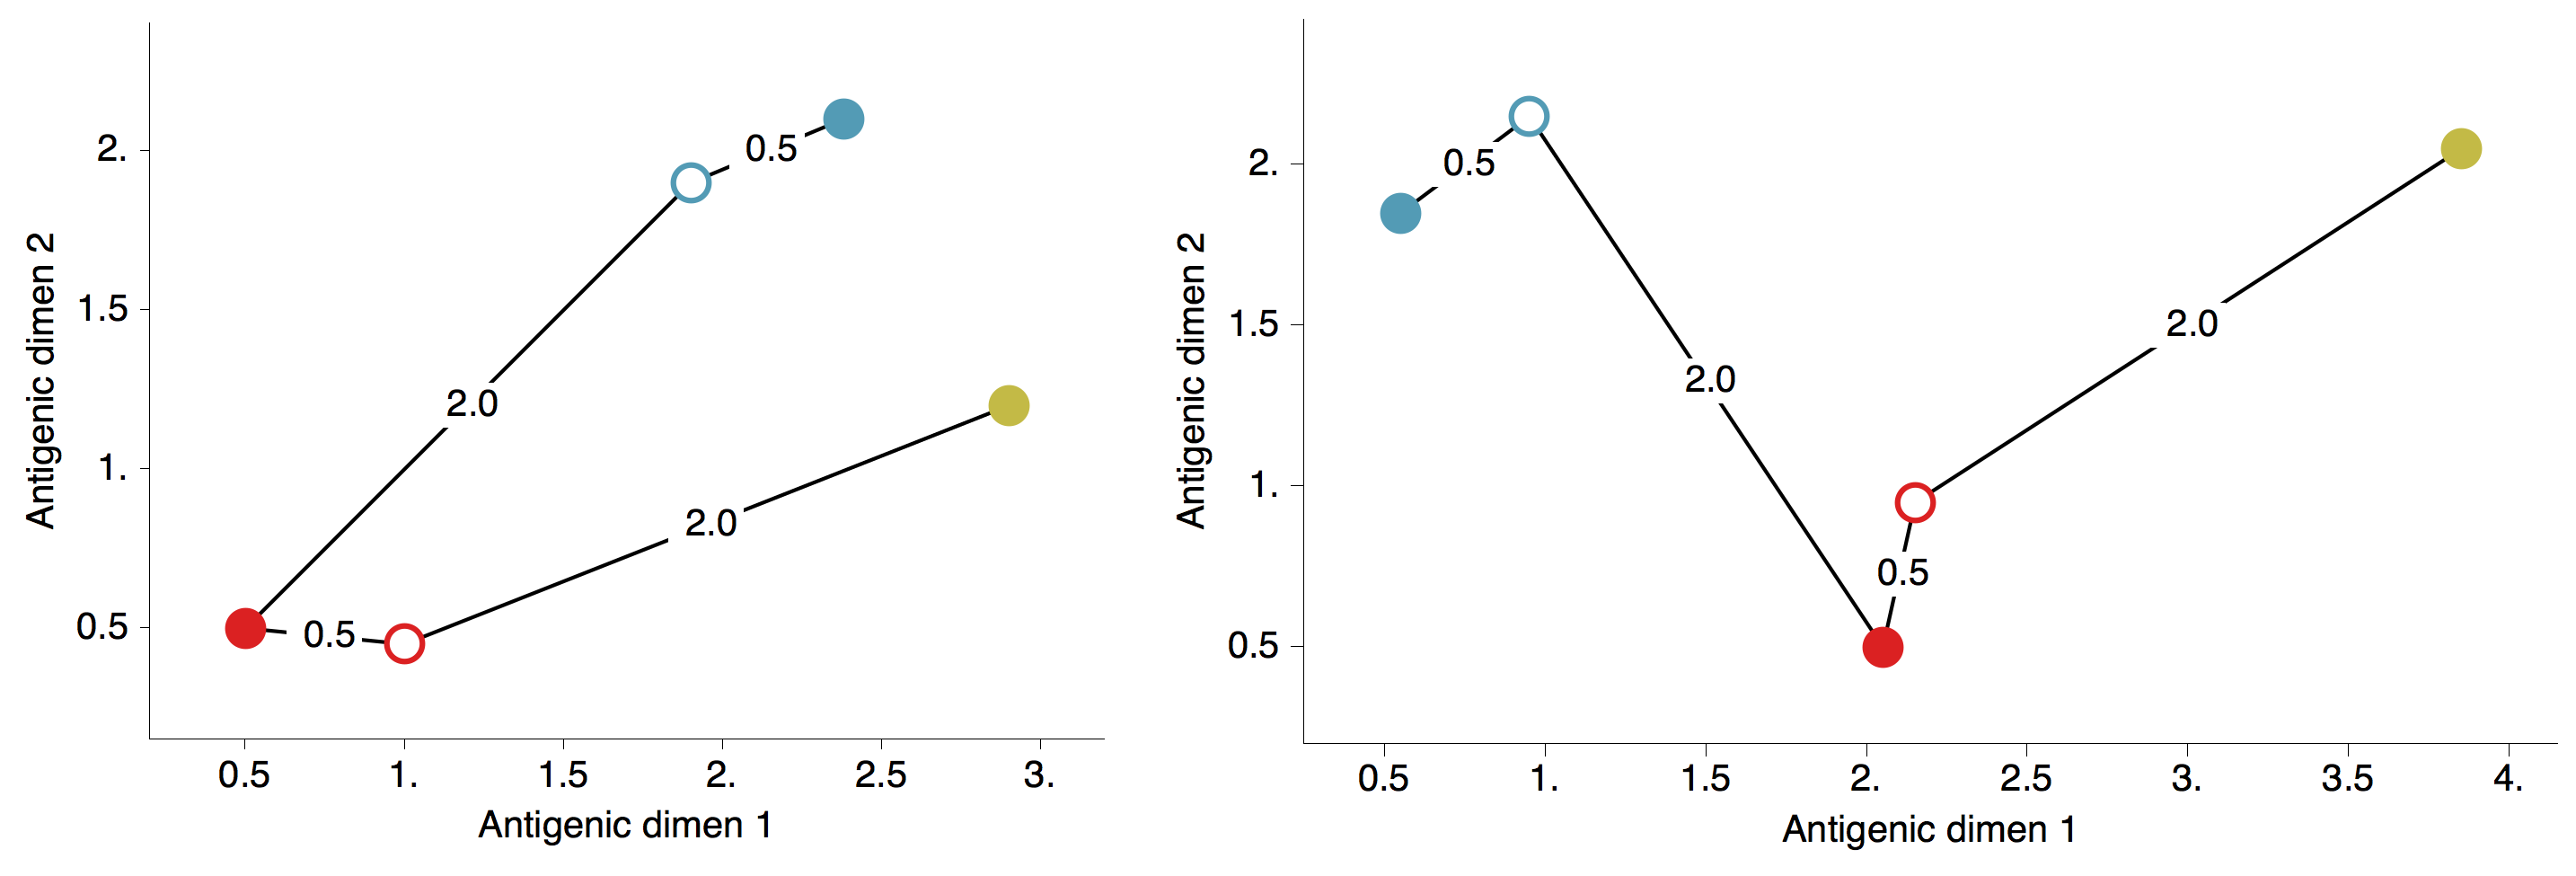
\includegraphics[width=0.95\textwidth]{figures/schematic_map}
	\caption{\textbf{Schematic antigenic map with three viruses and two sera.} 
	Virus 1 is shown in blue, virus 2 is shown in red and virus 3 is shown in yellow.
	Virus isolates are represented by filled circles, sera raised against viruses are shown as open circles and map distances $\delta_{ij}$ are shown as solid lines connecting viruses and sera.
	Sera from virus 1 is compared against viruses 1 and 2, while sera from virus 2 is compared against viruses 1 and 3.
	Left and right panels represent cartographic models that would give equal likelihoods of a given set of serological data $\{H_{11},H_{21},H_{22},H_{32}\}$.
	} 
	\label{schematic_map} 
\end{figure}

\subsection*{Diffusion model of antigenic evolution}

We simultaneously model antigenic locations and genetic relatedness by assuming that virus locations are influenced by evolution following a Brownian motion process \cite{Lemey10}.
To do this, we replace the previous prior specifying independent virus locations with a prior that incorporates covariance based on shared evolutionary history
\begin{equation} \label{ebpprior}
	\viruses \sim \left( \begin{matrix} \beta \, t_1 & 0 \\ \vdots & \vdots \\ \beta \, t_n & 0 \end{matrix} \right) + \, \mbox{Evolutionary Brownian Process}(\virussd, \tree)
\end{equation}
for $P=2$, where $\virussd$ is the volatility parameter of the Brownian motion and $\tree$ is a phylogeny specifying tree topology and branch lengths.
Thus, viruses which are genetically similar are induced to have prior locations close to one another on the antigenic map.
The evolutionary Brownian process assumes that the location $\node_i$ of node $i$ on the phylogeny follows from its parent node $p$, and with the addition of the drift along dimension 1, is distributed as
\begin{equation} 
	\node_i \sim (\beta \, d, \, 0)^{\prime} + \normal(\node_p, d \, \boldsymbol{\Sigma})
\end{equation}
for $P=2$, where $\node_p$ is the location of the parent node, $d$ is the length of the branch connecting nodes $i$ and $p$, and $\boldsymbol{\Sigma}$ is a diagonal matrix with diagonal elements all equal to $\virussd$.
The root node $\node_0$ is assumed to follow a normal distribution with expectation $(\beta \, t_0, 0)^{\prime}$ for $P=2$ and variance determined by the diffusion volatility $\virussd$ \cite{Lemey10}.
The probability of virus locations $p(\viruses | \beta, \virussd, \tree)$ is determined through analytical integration across internal states following the methods introduced in \cite{Lemey10}.
This formulation corresponds to a Weiner process with drift, in which the drift term $\beta$ only influences the expected states of nodes along the phylogeny, but does not influence the covariance structure among these nodes, which remains the same as it does in a standard Weiner process \cite{BrownianMotionHandbook}.
This allows the separation in equation \ref{ebpprior} between drift terms affecting only expectations and the evolutionary Brownian process that includes covariance among virus locations $\virus_1,\ldots,\virus_n$.

Here, the phylogenetic tree $\tree$ is estimated using sequence data for viruses $1,\ldots,\vn$ according to well established methods implemented in the software package BEAST \cite{BEAST17}.

\subsection*{Posterior samples}

Top-level priors for $1/\mdssd^2$, $\beta$, $1/\virussd^2$, and $1/\serumsd^2$ are assumed to follow diffuse $\mbox{Gamma}(a, b)$ distributions  with $a=0.001$ and $b=0.001$.
Under the full model, the posterior probability of observing virus and serum locations given immunological data is factored
\begin{equation}
	p(\viruses,\sera | \mathbf{H}) \propto p(\mathbf{H} | \viruses, \sera, \ses, \ves, \mdssd) \; 
	p(\viruses | \beta, \virussd, \tree) \;
	p(\sera | \beta, \serumsd) \; 
	p(\ses, \ves, \mdssd, \beta, \virussd, \serumsd, \tree).
\end{equation}
We sample from this posterior distribution using the Markov chain Monte Carlo (MCMC) procedures implemented in the software package BEAST \cite{BEAST17}.
Metropolis-Hastings proposals include transition kernels that translate individual virus and serum locations $\virus_i$ and $\serum_j$ and individual virus effects $\ve_i$ and serum effects $\se_j$, and other transition kernels that scale the entire set of virus and serum locations $\viruses$ and $\sera$ and that scale parameters $\mdssd$, $\beta$, $\virussd$ and $\serumsd$.
For the present analysis, a two-step approach was taken to sample phylogenies, where a posterior sample of phylogenies was gathered using sequence data and then, in the cartographic analysis, trees from this set were randomly proposed and accepted following the Metropolis-Hastings algorithm \cite{Pagel04}.

\subsection*{Data and implementation}

We compiled an antigenic dataset of hemagglutination inhibition (HI) measurements of virus isolates against post-infection ferret sera for influenza A/H3N2 by collecting data from previous publications and WHO vaccine strain selection reports (see Supp.\ Text).
Hemagglutinin sequences were compiled from the Influenza Research Database \cite{IRD} and the EpiFlu Database \cite{GISAID}.
Antigenic and genetic data were subsampled to give similar quantities of data across years of the analysis.
Data gathering procedures resulted in 402 virus strains A/H3N2, 115 virus strains for A/H1N1, 179 virus strains for B/Vic and 174 virus strains for B/Yam.
Surveillance data was obtained from the Centers of Disease Control and Prevention FluView Influenza Reports from the yearly summaries of influenza seasons 1997--1998 to 2010--2011 \cite{CDCReports}.

Phylogenetic trees were sampled for A/H3N2, A/H1N1, B/Vic and B/Yam using BEAST \cite{BEAST17} and incorporated the SRD06 nucleotide substitution model \cite{Shapiro06}, a coalescent demographic model with constant effective population size and a strict molecular clock across branches.
MCMC was run for 60 million steps and trees were sampled every 50,000 steps after allowing a burn-in of 10 million steps, yielding a total sample of 2000 trees.
These trees were treated as a discrete set of possibilities when subsequently sampled in the BMDS analysis \cite{Pagel04}.

MCMC was used to sample virus locations $\viruses$, serum locations $\sera$, virus effects $\ves$, serum effects $\ses$, MDS precision $1/\mdssd^2$, antigenic drift rate $\beta$, virus location precision $1/\virussd^2$, serum location precision $1/\serumsd^2$ and phylogenetic tree $\tree$.
MCMC chains were run for 500 million steps and parameter values sampled every 200,000 steps after a burn-in of 100 million steps, yielding a total of 2000 MCMC samples.

There is some difficulty summarizing posterior cartographic samples, as sampled virus and serum locations represent only relative quantities, and because of this, over the course of the MCMC, virus locations may shift.
Our prior on virus and serum locations removes much of this issue, orienting the antigenic map along dimension 1 and fixing it to begin at the origin.
However, local isometries are often still a problem.
For example, in A/H3N2 the Beijing/89 cluster may shift back and forth from being above other viruses on dimension 2 to being below other viruses on dimension 2.
These isometries may be local, i.e.\ Beijing/89 and Beijing/92 may flip while leaving Texas/77 in place.
Consequently, it is difficult to fully align MCMC samples using Procrustes analysis.
For the present study, we take a simple approach and sample a single MCMC step and visualize the antigenic locations at this state (Figures~\ref{map}, Figure~\ref{drift}).
Then, for specific quantities of interest, like rate of antigenic drift and rate of diffusion at different points along the phylogeny, we calculate this quantity across MCMC samples to yield an expectation and a credible interval.
This approach accurately characterizes uncertainty that may be hidden in an analysis of a single antigenic map.

\subsection*{Availability}

Source code implementing the cartographic models has been made fully available as part of the software package BEAST \cite{BEAST17}, and can be downloaded from its Google code repository (http://code.google.com/p/beast-mcmc/).
Antigenic, genetic and surveillance data is available as supplemental information \tbc{PREPARE}.

%%% ACKNOWLEDGMENTS %%%
\subsection*{Acknowledgments} 

We thank Richard Reeve, Dan Haydon, and Simon Frost for insights on antigenic modeling and MDS.
We acknowledge the laboratories that provided sequences to EpiFlu database: Centers for Disease Control and Prevention (USA), Chinese Center of Disease Prevention and Control, Hospital Clinic of Barcelona, National Institute of Hygiene of Morocco, National Institute of Infectious Diseases (Japan), National Institute for Medical Research (UK), Norwegian Institute of Public Health, Swedish Institute for Infectious Disease Control, Victorian Infectious Diseases Reference Laboratory (Australia).

%%% AUTHOR CONTRIBUTIONS %%%
\subsection*{Author contributions} 

AR, MAS, TB and PL conceived the study.
TB, GD, VG, AJH, JWM, CR, DS and AR gathered antigenic and genetic data.
AR, MAS, TB and PL designed statistical phylogenetic procedures.
TB performed the analysis.
TB, MAS and AR wrote the paper.

%%% FUNDING %%%
\subsection*{Funding} 

TB is supported by the Royal Society. 
MAS is supported by National Institutes of Health grants R01 GM086887 and R01 HG006139 and National Science Foundation grant DMS0856099.
VG, AJH and JWM are funded by MRC reference no U117512723.

%%% REFERENCES %%%
\bibliographystyle{plos}
\bibliography{flux}

\pagebreak

\setcounter{figure}{0}
\setcounter{table}{0}
%\setcounter{page}{1}
\renewcommand{\thefigure}{S\arabic{figure}}
\renewcommand{\thetable}{S\arabic{table}}
%\renewcommand{\thepage}{S\arabic{page}}

%%% SUPPORTING INFORMATION %%%
\section*{Supporting Information}

%%% error_by_distance_and_year %%%
\begin{figure}[H]
	\centering		
	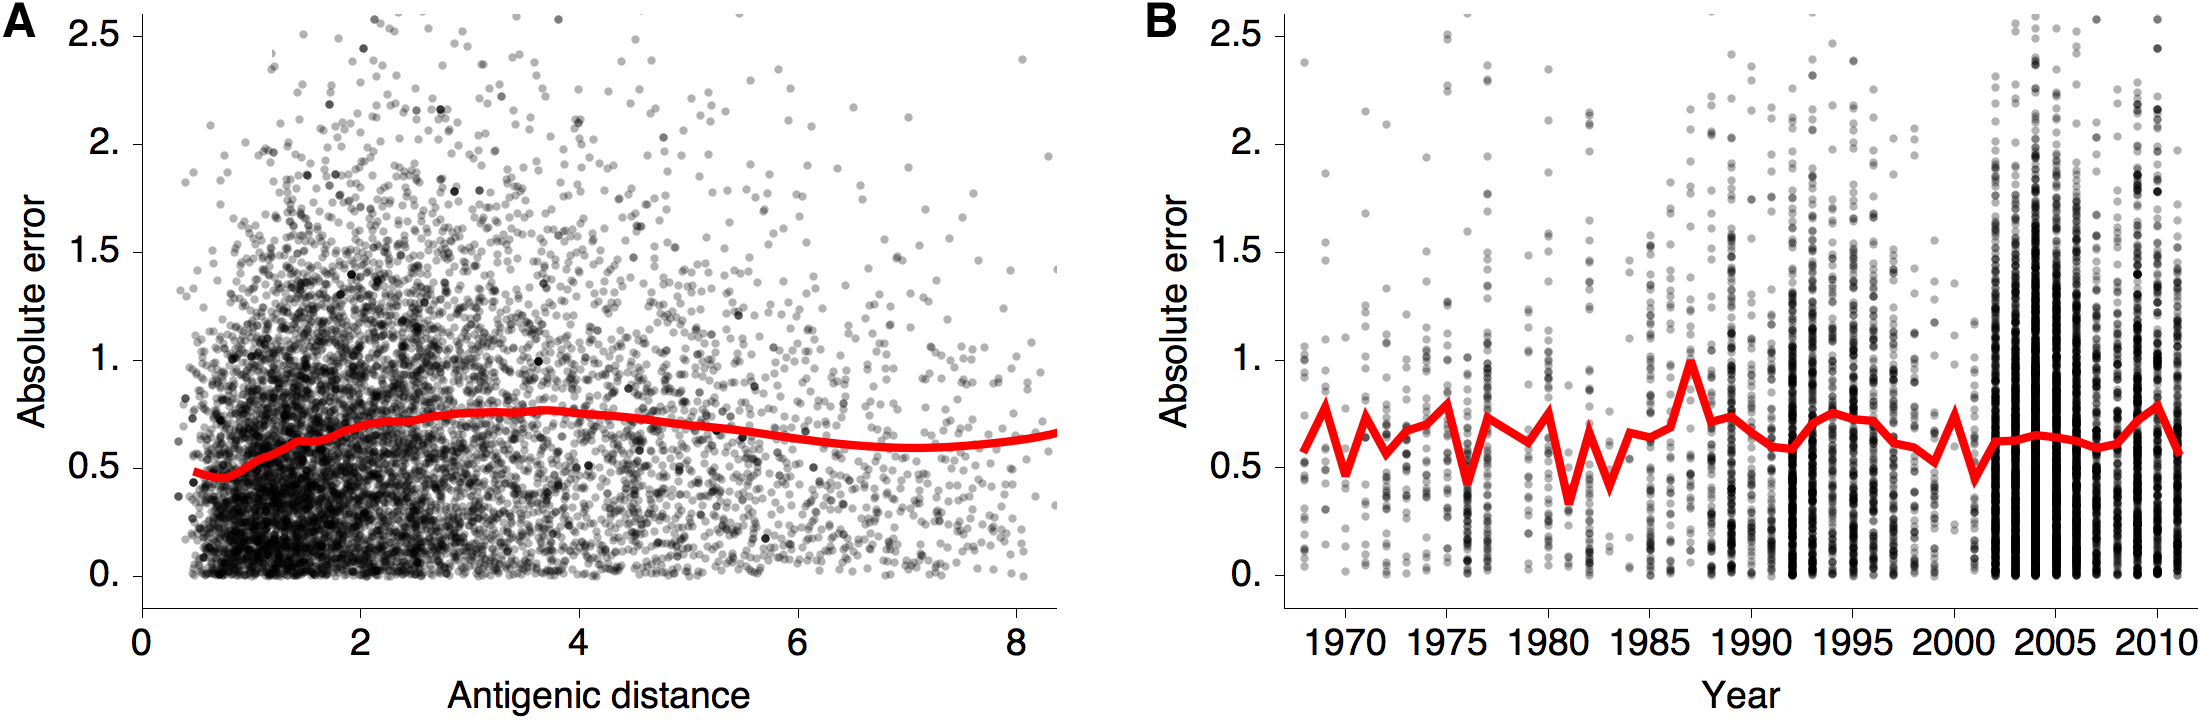
\includegraphics[width=0.95\textwidth]{figures/error_by_distance_and_year}
	\caption{\textbf{Absolute error in log$_2$ HI titer against antigenic distance and date of virus sampling in influenza A/H3N2.} 
	(A) Points show the absolute deviation from the predicted log$_2$ HI titer of the antigenic model, computed from virus location $\virus_i$, serum location $\serum_j$, virus effect $\ve_i$ and serum effect $\se_j$, based upon antigenic distance between virus and serum $\delta_{ij}$.
	The red line shows a LOESS regression curve of these points.
	(B) Points show the absolute deviation from the predicted log$_2$ HI titers of the antigenic model, based upon the date of virus sampling.
	The red line shows average deviations for each year.
	Relationships for A/H1N1, B/Vic and B/Yam are similar.
	} 
	\label{error_by_distance_and_year} 
\end{figure}

\end{document}
